\section{Implementering}
\subsection{Control (Styring)}
I Simpel Snake bruges kun fire taster til input, nemlig de fire piletaster, som derfor er defineret i \textit{Control}.\textit{Control}-klassen har metoden \textit{keyPressed}, som kommer af at \textit{Control}-klassen implementerer \textit{KeyListener}, som kaldes hver gang der tastes på tastaturet. Hvis tasten er en af de fire piletaster, kaldes funktionen \textit{move} i \textit{Snake}-klassen, der flytter hovedet i samme retning som piletasten.
Enum-klassen \textit{Direction} indholder \textit{RIGHT, LEFT, UP} og \textit{DOWN}. Dette bruges i \textit{Control}-klassen, da det ikke skal være muligt at bevæge sig i modsatte retning af slangens nuværende retning.
I \textit{Control}-klassens constructor er Direction som udgangspunkt sat til \textit{LEFT}, da slangen starter mod venstre. Hver gang der tastes på piletasterne, sikrer \textit{keyPressed}-metoden, at retningen ikke er modsat af den nuværende retning. Herefter flyttes slangen, uanset om den er midt på spillepladen eller om den bevæger sig rundt om torussen. Til sidst sættes \textit{Direction} til den nuværende retning, så det ved næste tasteanslag igen kan undersøges, at retningen ikke er modsat.

\subsection{Model}
Spillets model består af en række klasser, der tilsammen udgør selve spillets funktioner og objekter.
Klassen \textit{Field} bruges til at definere et et punkt, som repræsenterer et felt i banen. Den fungerer på samme måde som \textit{Point}-objekt-klassen, hvor koordinatsystemet starter oppe i venstre hjørne. Forskellen mellem \textit{Point}- og \textit{Field}-klassen, er hvordan man kommer frem til et punkt. \textit{Point}-klassen går først ud ad x-aksen og derefter ned ad y-aksen, hvorimod \textit{Field}-klassen gør det i omvendt rækkefølge. Da hele spillepladen er delt op i rækker og kolonner, frem for en x- og y-akse, er \textit{Field} lettere at bruge for at undgå forvirring, dato-dimensionelle arrays også er opdel i rækker og kolonner, hvor den første værdi repræsenterer rækker, mens den anden værdi repræsenterer kolonner..

Funktionenen \textit{equals} er defineret i denne klasse, og bruges til at undersøge om to objekter ligger på samme felt, f.eks. slangens hoved og æblet. Æblet bliver oprettet i klassen \textit{Game}, hvor datafeltet \textit{position} afgør dets nuværende position.

Slangen selv er defineret i klassen \textit{Snake}. Slangens krop består af en række felter, hvoraf det første er hovedet, og de resterende er kroppen inklusiv halen til sidst. Koordinaterne for disse felter er gemt som elementer i en ArrayList kaldet \textit{positions}. Det første element er slangens første led, hovedet, det andet element er slangens andet led osv. Når et nyt led tilføjes, tilføjes et nyt element til listen. Dette sker, når slangen spiser et æble, hvor den ikke bevæger sig som ellers. I stedet tilføjes et nyt hoved på æblets felt. Hovedets retning er den samme, som slangens sidste bevægelse.

I \textit{Snake}-constructoren bliver slangens hoved og hale oprettet, hvor hovedet bliver placeret i banens centrum. Halen placeres i kolonnen til højre for på samme række.

I \textit{move}-metoden benyttes Action-klassen, der er oprettet som en enum, og betegner slangens handlinger: om slangen spiser et æble, er død eller bevæger sig (hhv. \textit{EAT, KILL, MOVE}). I \textit{move}-metoden undersøges der, om der er mad på samme felt som hovedets nye placering. Er dette tilfældet, bliver Action-statementet til \textit{EAT}. Hvis ikke, undersøges der om den nye placering for hovedet allerede indeholder slangens krop. Gør der det, bliver Action-statementet til \textit{KILL}. Hvis ikke, flyttes slangens hoved til den nye position. Resten af slangens krop følger med ved at ændre koordinaterne i \textit{positions} fra halen og op til hovedet, dvs. at halens koordinater bliver næstsidste led, næstsidste bliver tredjesidste osv. Slangens krop flyttes først, hvorefter hovedet flyttes til sidst, for at undgå at andet led indtager samme plads som hovedet.

I \textit{Game}-klassen findes \textit{checkAction}-metoden, der undersøger om slangen spiser eller dør. Hvis Action-statementet er \textit{EAT}, øges slangens længde ved at tilføje et nyt element på æblets felt, som fungere som nyt hoved. Scoren inkrementeres, der laves et nyt æble, og Action-statementet sættes til \textit{MOVE}.
Hvis Action-statementet er \textit{KILL}, nulstilles scoren, og spillet slutter ved at slangen ikke længere kan bevæge sig.
Herudover findes \textit{generateFood}-metoden, som sikrer, at maden altid placeres på et gyldigt felt, dvs. et felt der ikke er udfyldt af slangen. For at sikre dette, placeres æblet på et tilfældigt felt inden for banens rammer, hvorefter der undersøges om et af slangens led har samme koordinater som æblets felt. Er dette tilfældet, gives æblet et nyt felt, indtil det lander på et felt uden slangen. Er slangen tilpas stor, er dette dog ikke effektivt, da der er stor sandsynlighed for at ramme et felt, der er optaget af slangen. Af denne årsag undersøger metoden først, om slangen fylder mere end halvdelen af banen. Er dette tilfældet, laves der i stedet en liste med alle tomme felter vha. en indlejret for-løkke, der løber gennem alle række og kolonner, hvorefter et tilfældigt element i listen vælges som æblets position.

De fire klasser \textit{Food, Score, Game} og \textit{Snake} forlænger klassen \textit{Observable}, så det er muligt for View at modtage ændringerne i \textit{Model}, uden at \textit{Model} afhænger af View.

\subsection{View (Brugergrænseflade)}
Brugerfladen er samlet i klassen \textit{GameView} der forlænger \textit{JFrame}. I \textit{GameView} findes kun en constructor, hvor der oprettes et \textit{ScorePanel}-objekt, der placeres øverst i vinduet, og et \textit{BoardPanel} objekt, der placeres direkte under det. Board-panelet viser selve banen med slangen og æblet, der begge er vist ved farvede firkanter. 

\textit{ScorePanel}-klassen forlænger \textit{JPanel} og implementerer \textit{Observer}. Klassen har en \textit{update}-metode, der gentegner, hver gang noget ændrer sig i de klasser i model-pakken, der forlænger \textit{Observable}. 
\textit{paintComponent}-metoden benyttes til at tegne score-teksten. Selve panelet oprettes i constructoren.

\textit{BoardPanel} forlænger også \textit{JPanel} og implementerer \textit{Observer}, for at den også kan registerere ændringer i model-klasserne. \textit{BoardPanel} består af en række draw-metoder, samt en \textit{paintComponent}-metode, der kalder på draw-metoderne for at tegne alle spillets komponenter på spillets bane og spillets bane selv.
I \textit{drawSnake}-metoden bruges positionerne for slangens felter til at tegne slangen. Størrelsen for et felt udregnes i \textit{getWindowRectangle}-metoden, og afhænger af vinduets og banens størrelse. Når feltets størrelse er udregnet, tegnes en rektangel med feltets størrelse på alle felterne i slangens positions-ArrayList.

\section{Udviklingsproces}
\subsection{Arbejdsproces}
Formålet med projektet var at starte med at lave en simpel udgave af snake, og derefter tilføje flere funktioner for at lave en mere avanceret version. Dette gør det ideelt at tilføje én funktion ad gangen, frem for at planlægge alle funktioner på en gang, og tilføje dem samtidig. Resultatet bliver et, til at starte med, simpelt men fungerende program, hvorefter yderligere funktioner kan tilføjes. Programmet er altså udviklet iterativt, hvorved der opstår flere fungerende versioner af spillet, men med forskellige funktioner. Dette gør det muligt at tilpasse programmet, hvis der opstår nye idéer eller krav undervejs. 

Den iterative tilgang gør det muligt at have en "cyklus" for udviklingen af programmet. Først bestemmes det, der skal tilføjes til programmet. Derefter fordeles opgaverne blandt gruppens medlemmer. Gruppemedlemmet afgør selv, hvordan en funktion skal designes og implementeres, men sikrer at implementationen er kompatibel med alle nuværende funktioner, og ikke vil hindre fremtidige tilføjelser i at blive tilføjet. Eventuelle justeringer til programmet laves for at undgå fejl med nye funktioner, hvorefter "cyklussen" starter forfra ved idéfasen.

\subsection{Control}
Idet der ikke er brug for nogen menu eller lignende i Simpel Snake, er det muligt at holde styringen af spillet meget simpel. Ved at definere de fire piletaster i \textit{Control}-klassen, samt en funktion til at sikre at der ikke bevæges i modsat retning, er alle styringkrav til Simpel Snake opfyldt. Resten af spillet håndteres da i model-koden.

\subsection{Model}
\subsubsection{Opbygning af banen}
Til designet af banen, som slangen bevæger sig på, foreslås to muligheder. Den ene er at lave et to-dimensionelt array af datatypen enum, hvis størrelse afgør banens endelige størrelse. Et array [10][5] vil f.eks. give en bane med længden 10 og bredden 5. Hvert element i arrayet bestemmer da, hvad der befiner sig på netop denne plads på banen. Elementerne i arrayet kan f.eks. være et blankt felt, et æble, et led af slangen osv. Dette gør det nemt at introducere nye spilelementer i fremtiden, f.eks. bonus-point, vægge og miner, idet der blot skal tilføjes nye værdityper. Visualisering af spillet foregår ved at definere et billede for hvert spilelement, og få programmet til at tegne objektet på arrayets plads.

En anden metode er, at lade de forskellige spilelementer være defineret i deres egne klasser, så f.eks. \textit{SnakeFood} er en klasse for sig selv, \textit{SnakePlayer} er en klasse for sig selv osv. Hver klasse har de funktioner, der er relevante for dem, f.eks. \textit{getPosition} for at give deres nuværende position. Programmet tegner da spillet hver gang en tur afsluttes, dvs. når alle elementer som skal ændres, er ændret. Programmet har fået defineret billedet for de forskellige elementer, og modtager deres position vha. en \textit{getPosition} metode.
Ulempen ved denne metode er, at det skal laves flere metode og klasser, hvormed programmets kompleksitet stiger. I den første metode er alle felter allerede defineret, og for at ændre dem behøves værdien for hvert felt blot at blive ændret, så f.eks. et blankt felt ændres til æble. Ønskes et spilelement ændret eller introduceret med den anden metode, skal der laves et nyt objekt. Ønsker man at introducere nye elementer, kan man med første metode blot tilføje en ny værdi-type til det todimensionelle array. Med anden metode skal der laves nye klasser, metoder osv. for at introducere nye elementer til spillet.
 
I sidste ende blev metode 2 valgt, idet den gjorde det nemmere at holde Model-koden adskilt fra View- og Control-koden. Herudover har første metode den ulempe, at den skal sende et todimensionelt array på banens størrelse, hver gang banen skal tegnes. Ved en bane på f.eks. 100x100 betyder dette, at at sendes i alt 10000 elementer til View-koden, hver gang banen skal tegnes. Den anden metode sender derimod kun de relevante elementer, dvs. æblets og slangens position, til View-koden.

\subsubsection{Snake}
Da slangen i snake-spillet består af en række felter, som alle har netop en koordinat i forbindelse med andre led, er en effektiv måde at bestemme slangens position på en ArrayList, idet denne datastrukturer er fleksibel i størrelse og passer til formålet. Når slangen vokser i størrelse, bliver dette dog mindre effektivt, idet slangens hoved altid sættes som element 0. Når slangen vokser, tilføjes et nyt element på plads 0, hvormed hele listen skal flyttes. En anden mulighed ville være at bruge en anden datastruktur, f.eks. LinkedList, eller lade hovedet være defineret som element positions.size()-1, hvormed nye hovedet tilføjes sidst i listen. Et problem ved at bruge LinkedList er dog, at denne datastruktur ikke tillader vilkårlig adgang af værdier, men derimod altid bevæger sig fra første eller sidste element. Dette problem kan løses ved at bruge en iterator, men blev fravalgt, idet det skabte problemer, når listen skulle bruges på tværs af klasserne.

Til implementationen af scoren blev to løsninger foreslået. Enten at lade scoren være et datafelt i game-klassen, eller at lade det være en klasse for sig selv. Ved at lade scoren være et datafelt, bliver implementationen simplere. At lade scoren være en klasse for sig selv har derimod fordelen, at der kan 
tilføjes en observer til Score-klassen, som dermed kun opdateres, når scoren ændrer sig. Scorepanelet tegnes ikke i samme klasse som banen, og kan derfor holdes seperat, så scorepanelet kun gentegnes, når scoren ændrer sig. Hvis scoren derimod er et datafelt, tegnes scoren efter hver tur, også selvom scoren er uændret. I sidste ende blev det bestemt at holde scoren som datafelt, hvormed fremtidige score-relaterede funktioner bliver simplere at implementere.

\subsection{Brugerflade og visualisering af programmet}
\subsubsection{Tegning af spillet}
For at visualisere spillet er det nødvendigt at kunne optegne banen, slangen og æblet. Dette gøres i klassen ViewBoard, som har metoderne drawBackground, drawBoard, drawSnake og drawFood, som hver især tegner deres tilsvarende element. Metoden paintComponent kalder de førnævnte metoder, således at baggrunden tegnes først, så banen, så æblet og sidst slangen. Alting gentegnes hver gang spillet opdateres, hvormed der "tegnes over" det gamle billede. Det kan her argumenteres for, at f.eks. baggrunden ikke bør gentegnes, når slangen bevæger sig, lige som store dele af banen forebliver uændret, og derfor ikke behøver gentegnes. Alternativt kunne man lave et system, som undersøger hvilke områder der skal gentegnes, og hvilke der er uændret, og derfor ikke skal gentegnes. Dette kan dog i sidste ende betyde, at de kræfter der spares på tegning i stedet blot bruges på at afgøre, hvad der skal tegnes.

\subsubsection{Vinduesstørrelse}
Området, som spillet foregår på, skal kunne bestemmes til at være mellem 5x5 og 100x100. Dette kan dog skabe problemer, hvis størrelsen bliver for stor, idet banen både skal være synlig, men også passe på en gennemsnitlig computerskærm. En bane på 10x10 kan sagtens passe på en opløsning af f.eks. 400x400, men øges banens størrelse til 50x50, bliver banen svær at se. Herudover varierer skærmstørrelser, og det er derfor nødvendigt at gøre spillets vinduestørrelse fleksibel. En løsning på dette problem ville være at bestemme en fast størrelse for felterne, og lade vinduet justere sin størrelse efter dette. Ønskes det f.eks. at felterne altid har størrelsen 20x20, og at banen skal være 15x25, vil vinduets størrelse blive 300x500. Fordelen ved denne metode er at det sikres, at banen altid er synlig, og at der ikke opstår problemer, fordi forholdet mellem vinduets størrelse og banen størrelse ikke passer sammen. Ulempen ved metoden er, at store baner kan blive for store til at være på en normal skærm. F.eks. vil en bane med felter af størrelsen 20x20 og banestørrelsen 75x75 fylde 1500x1500. Herudover er løsningen ikke brugervenlig, idet en bruger kan blive forvirret over hvorfor vinduets størrelse ændrer sig fra bane til bane, og måske ligefrem ikke passer på skærmen.

En anden metode er at gøre vinduet justerbart. Denne løsning er mere brugervenlig, idet vinduets størrelse frit kan justeres så det passer til den enkelte person. Denne metode introducerer dog et andet problem, nemlig at felternes størrelse skal skaleres til at passe vinduet. Nogle opløsninger af vinduet vil ikke være et multiplum af banens størrelse, hvormed elementerne i spillet vil blive aflange. Dette problem bliver løst i avanceret snake ved at lave en baggrund og låse banens forhold, hvormed banen altid fylder mest muligt af vinduet ud, mens den beholder sin form, og den resterende plads bliver udfyldt af baggrunden. Idet denne løsning var nemmere at bruge og forstå, og giver bedre mulighed for justering af spillet, blev den valgt frem for den første løsning.
\begin{figure}[h]
	\centering
	\graphicspath{ {pics/} }
	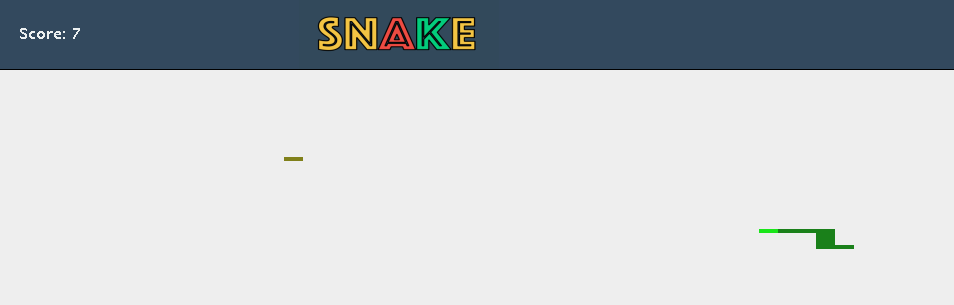
\includegraphics[width=0.5\textwidth]{WindowSize.png}
	\label{fig:windowsize}
	\caption{windowsize}
\end{figure}